\chapter{Kernel FDA with Multi-layer Kernels}
\label{chap_kfda}
In this chapter we study the discriminating power of multi-layer kernels with kernel Fisher Discriminant Analysis(KFDA\nomenclature{KFDA}{Kernel Fisher Discriminant Analysis}). The analysis in this section was done on binary classification problems. This chapter is organized as follows: section \ref{chap4_kfda} gives a brief introduction of kernel Fisher discriminant Analysis, section \ref{chap4_experiment} contains the results of empirical study on \textit{rectangles-image} and \textit{convex} datasets(both are binary classification problems studied extensively in deep learning literatures), and section \ref{chap4_conc} gives the conclusion.  

\section{Kernel Fisher Discriminant Analysis}
\label{chap4_kfda}
The working principle of discriminant analysis is to find a set of features that discriminates the classes very well(\cite{kfda} et al.). Fisher Discriminant Analysis(FDA) was originally proposed for learning a set of discriminating features in the input space. Kernel FDA is a non-linear generalization of FDA, in which the discriminating features are learned in feature space.

Let $X_1 = \{x_1^1, \ldots, x_{n_1}^1 \}$ and $X_2 = \{x_1^2, \ldots, x_{n_1}^2 \}$ be data samples from two classes (class 1 and class 2) and the union of two, denoted as $X = X_1 \cup X_2$ as the training set.  KFDA find the directions $f$ which maximizes the cost function

\begin{equation}
\mathcal{J}(f) = \frac{f^TS_B^{\phi}f}{f^TS_W^{\phi}f} 
\label{4_jw}
\end{equation}

where $f \in \mathcal{F}$ and $S_B^{\phi}$ and $S_W^{\phi}$ are the between and within class scatter matrices respectively
\[ S_B^{\phi} = (m_1^{\phi} - m_2^{\phi})(m_1^{\phi} - m_2^{\phi})^T \]
\[ S_W^{\phi} = \sum_{i=1,2}\sum_{x \in X_i} (\phi(x)-m_i^{\phi})(\phi(x)-m_i^{\phi})^T  \]
where $m_i^{\phi} = \frac{1}{n_i} \sum_{j=1}^{n_i} \phi(x_j^i)$. Intuitively maximizing $\mathcal{J}(f)$ is equivalent to finding a direction $w$ which maximizes the separation of the two classes while minimizing the within class variance(\cite{kfda} et al.). We need to transform the formulation in \ref{4_jw} in terms of kernel function $k(x, y) = \phi(x) \cdot \phi(y)$ in order to use kernels. According to RKHS\nomenclature{RKHS}{Reproducing Kernel Hilbert Space} theory, any solution to the Tikhnov regularization $f \in \mathcal{F}$ must lie in the span of the feature map($\phi(\cdot)$) corresponding to training examples. Thus it can be represented as
\begin{equation}
f = \sum_{i=1}^n \alpha_i \phi(x_i)
\label{4_wrkhs}
\end{equation}
combining \ref{4_wrkhs} and the definition of $m_i^{\phi}$ we have
\[ f^Tm_i^{\phi} = \frac{1}{n_i} \sum_{j=1}^n \sum_{k=1}^{n_i} \alpha_j k(x_j, x_k^i) = \alpha^T M_i \]
where $(M_i)_j = \frac{1}{n_i} \sum_{k=1}^{n_i}  k(x_j, x_k^i)$. Define $M = (M_1-M_2)(M_1-M_2)^T$. The we have
\begin{equation}
f^T S_B^{\phi} f = \alpha^T M \alpha
\label{4_wsbw}
\end{equation}
using similar transformations we have
\begin{equation}
f^T S_W^{\phi} f = \alpha^T N \alpha
\label{4_wsww}
\end{equation}
where $N = \sum_{i=1,2} K_i(I - \bm{1}_{n_i})K_i^T $, $K_i$ is an $n \times n_i$ matrix with entries $(K_i)_{nm} = k(x_n, x_m^i)$(this is the kernel matrix for class $i$), $I$ is the identity matrix and $\bm{1}_{n_i}$ is the matrix with with all entries $\frac{1}{n_i}$. The derivation of this compact forms $M$ and $N$ are shown in Appendix \ref{derivation2}.

Combining (\ref{4_wsbw}) and (\ref{4_wsww}) we will get an objective function in terms of $\alpha$.
\[ \mathcal{J}(\alpha) = \frac{\alpha^T M \alpha}{\alpha^T N \alpha}  \]
This problem can be solved by finding the leading eigen vectors of $N^{-1}M$. The projection of a new pattern $x$ onto $f$ is given by
\[ f \cdot \phi(x) = \sum_{i=1}^n \alpha_i k(x_i, x) \]
The estimation of $N \in \mathbb{R}^{n \times n}$ from a sample of size $n$ poses an ill-posed problem(since the sample size is not high enough to get an exact covariance structure in $\mathbb{R}^{n \times n}$). This problem is solved by replacing $N$ with $N_{\mu}$ as
\[ N_{\mu} = N + \mu I \]
where $\mu$ is a large positive constant and $I$ is the identity matrix. This has two possible benefits
\begin{itemize}
\item It makes the problem numerically more stable as for large $\mu$, $N_{\mu}$ will become positive definite.
\item It decreases the bias in sample based estimation of eigenvalues.
\end{itemize}


\section{Experiments}
\label{chap4_experiment}
Empirical study was conducted on two binary classification datasets namely \textit{rectangles-image} dataset and \textit{convex} dataset. A short description about \textit{rectangles-image} dataset is given in \autoref{chap_mkm}.
\subsection{Convex Dataset}
The \textit{convex} dataset consists of a single convex region in an image. The dataset was constructed by taking the intersection of a number of half-planes whose location and orientation were chosen uniformly at random. The classification task was to identify whether the shape enclosed in the image is convex or not. This dataset consists of 12000 training and 50000 testing samples of size 28$\times$28.

Figure \ref{shape} shows some sample images from \textit{rectangles-image} and \textit{convex} datasets. In the experiments, KFDA with multi-layer arc-cosine kernels were used for feature extraction and kNN classifier was used for the classification. Table \ref{kfda_results} shows the results of the empirical study.

\begin{figure*}
  \centering
  \captionsetup{justification=centering,margin=0.1cm}
  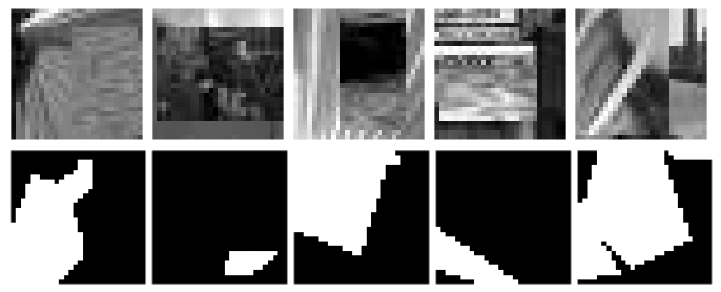
\includegraphics[scale=0.6]{figures/shapes}
  \caption{Sample images from \textit{rectangles-image}(first row) and \textit{convex}(second row) datasets.}
  \label{shape}
\end{figure*}

\renewcommand{\arraystretch}{2.3}
\begin{table*}
\centering
\begin{tabular}{|c|c|c|c|c|c|c|c|}
  \hline
  \multirow{2}{*}{\textbf{Dataset}} & \multicolumn{7}{ |c| }{\textbf{Loss in Percentage}} \\
  \cline{2-8}
  &$\textrm{SVM}_{\textrm{RBF}}$ & $\textrm{SVM}_{\textrm{Poly}}$ & NNet & DBN-3 & SAA-3 & DBN-1 & \textbf{KFDA}\\
  \hline  
  \textit{rect-image} & 24.04 & 24.05 & 33.20 & 23.69 & 24.05 & 22.50 & \textbf{21.96}\\
  \hline
  \textit{convex} & 19.13 & 19.82 & 32.25 & 19.92 & \textbf{18.41} & 18.63 & 19.02\\
  \hline
\end{tabular}
\caption{Experimental Results of KFDA with multi-layer kernels.}
\label{kfda_results}
\end{table*}
\renewcommand{\arraystretch}{1}

\renewcommand{\arraystretch}{2}
\begin{table}
\centering
\begin{tabular}{|c|c|}
  \hline
  \textbf{Kernel Parameters} &  \textbf{Loss in Percentage}\\
  \hline
  0 & 23.12\\
  \hline
  0,3 & 22.54\\
  \hline
  0,3,3 & 22.39\\
  \hline
  0,3,3,3 & 22.15\\
  \hline
  0,3,3,3,3 & 21.96\\
  \hline
  0,3,3,3,3,3 & 22.01\\
  \hline  
\end{tabular}
\caption{Change in classifier performance while increasing number of layers for \textit{rectangles-image} dataset}
\label{chap4_tab1}
\end{table}
\renewcommand{\arraystretch}{1}

\renewcommand{\arraystretch}{2}
\begin{table}
\centering
\begin{tabular}{|c|c|}
  \hline
  \textbf{Kernel Parameters} &  \textbf{Loss in Percentage}\\
  \hline
  1 & 21.94\\
  \hline
  1 $\times$ 3 & 21.68\\
  \hline
  1 $\times$ 6 & 21.46\\
  \hline
  1 $\times$ 9 & 19.78\\
  \hline
  1 $\times$ 12 & 19.52\\
  \hline
  1 $\times$ 15 & 19.38\\
  \hline
  1 $\times$ 18 & 19.30\\
  \hline
  1 $\times$ 21 & 19.02\\
  \hline      
\end{tabular}
\caption{Change in classifier performance while increasing number of layers for \textit{convex} dataset}
\label{chap4_tab2}
\end{table}
\renewcommand{\arraystretch}{1}

For \textit{rectangles-image} dataset, the best result was obtained for a five layer KFDA with kernel degree values in each layer was given by [0,3,3,3,3]. For \textit{convex} dataset the best result was obtained from a model having 20 layers with degree parameter equal to 1 in each layer. The variations in classifier performance as the number of layers were increased is shown in tables \ref{chap4_tab1} and \ref{chap4_tab2} for \textit{rectangles-image} and \textit{convex} datasets respectively. In table \ref{chap4_tab2}, 1 $\times$ $n$ indicates that an arc-cosine kernel of $n$ layers is used with kernel parameter is equal to `1' in each layer.


\section{Conclusion}
\label{chap4_conc}
In this chapter we experimented on KFDA with multi-layer arc-cosine kernels. The result obtained are very promising. On \textit{rectangles-image} dataset, the classifier performed even better than a DBN based model. On \textit{convex} dataset, its performance was better than all shallow models 
and was comparable with that of deep models. One of the striking observation from these results is that, better performance is obtained when using either a highly non-linear arc-cosine kernel(degree $>$ 1) or a multi-layer arc-cosine kernel with very large number of layers (above 10).
